%%%%%%%%%%%%%%%%%%%%%%%%%%%%%%%%%%%%%%%%%
% Beamer Presentation
% LaTeX Template
% Version 1.0 (10/11/12)
%
% This template has been downloaded from:
% http://www.LaTeXTemplates.com
%
% License:
% CC BY-NC-SA 3.0 (http://creativecommons.org/licenses/by-nc-sa/3.0/)
%
%%%%%%%%%%%%%%%%%%%%%%%%%%%%%%%%%%%%%%%%%

%----------------------------------------------------------------------------------------
%	PACKAGES AND THEMES
%----------------------------------------------------------------------------------------

\documentclass[c]{beamer}
%\documentclass[notes]{beamer}
\setbeamertemplate{note page}[show only notes]
\input{../OR_common.tex}
%%%%%%%%%%%%%%%%%%%%%%%%%%%%%%%%%%%%%%%%%%%%%%%%%%%%%%%%%%%%%%%%%%%%%%%%%%%%%
%%%%%%%%%%%%%%%%%%%%%%%%%%%%%%%%%%%%%%%%%%%%%%%%%%%%%%%%%%%%%%%%%%%%%%%%%%%%%
%%%%%%%%%%%%%%%%%%%%%%%%%%%%%%%%%%%%%%%%%%%%%%%%%%%%%%%%%%%%%%%%%%%%%%%%%%%%%

\title[Introduction]{Unit 2. Linear programming. Duality}

\author{Jordi Villà i Freixa}
\institute[FCTE]{
Universitat de Vic - Universitat Central de Catalunya \\
Study Abroad. Operations Research\\
\medskip
\textit{jordi.villa@uvic.cat}
}
\date{April 18th, 2024}
\logo{
\includegraphics[width=.1\textwidth]{FCTE}}
\begin{document}

\begin{frame}
\titlepage
\end{frame}


\begin{frame}
    \frametitle{Preliminary}
    This course is strongly based on the monography on Operations Research by Carter, Price and Rabadi \cite{carter}, and in material obtained from different sources (quoted when needed through the slides).
\end{frame}

%%%%%%%%%%%%%%%%%%%%%%%%%%%%%%%%%%%%%%%%%%%%%%%%%%%%%%%%%%%%%%%%%%%%%%%%%%%%%
%%%%%%%%%%%%%%%%%%%%%%%%%%%%%%%%%%%%%%%%%%%%%%%%%%%%%%%%%%%%%%%%%%%%%%%%%%%%%
%%%%%%%%%%%%%%%%%%%%%%%%%%%%%%%%%%%%%%%%%%%%%%%%%%%%%%%%%%%%%%%%%%%%%%%%%%%%%

\begin{frame}
\frametitle{Learning outcomes}
\begin{itemize}
  \item Understanding Dual and Primal problems in LP
  \item Economic interpretation
  \item Conditions of optimality
  \item Resolution of the dual by the primal and penalty method
\end{itemize}
\end{frame}

\section{Duality}
\note{\url{https://www.youtube.com/watch?v=yU8updOR87c}}
\begin{frame}[allowframebreaks]{A first example}

  Linear programming problems come in pairs!

  \begin{equation*}
    \begin{aligned}
      \text{maximize  } \quad & 4x_1 + x_2 +5x_3 +3x_4 \\
      \text{subject to }\quad &
      \left\{
      \begin{array}{rcl}
        x_1 - x_2 -x_3 +3x_4 &\leq &1 \\
        5x_1 + x_2 +3x_3 +8x_4 &\leq &55 \\
        -x_1 + x_2 +3x_3 -5x_4 &\leq &3 \\
        x_1,x_2,x_3 &\geq& 0
      \end{array}
      \right.
    \end{aligned}
  \end{equation*}

note that
\begin{eqnarray*}
  y_1(x_1 - x_2 -x_3 +3x_4)&+&\\y_2(5x_1 + x_2 +3x_3 +8x_4)&+&\\y_3(-x_1 + x_2 +3x_3 -5x_4) &\leq& y_1+55y_2+3y_3
\end{eqnarray*}

\end{frame}
\begin{frame}{Primal and Dual}

We see that maximizing the {\bf Primal objective function} $4x_1 + x_2 +5x_3 +3x_4$ is
  equivalent to minimize the {\bf Dual objective function} $y_1+55y_2+3y_3$:

    \begin{equation*}
    \begin{aligned}
      \text{minimize } \quad & y_1+55y_2+3y_3 \\
      \text{subject to }\quad &
      \left\{
      \begin{array}{rcl}
        y_1 + 5y_2 -y_3 &\geq &4 \\
        -y_1 +y_2 +y_3 &\geq &1 \\
        -y_1 +3y_2 +3y_3 &\geq &5 \\
        3y_1 +8y_2 -5y_3 &\geq &3 \\
        y_1,y_2,y_3,y_4 &\geq& 0
      \end{array}
      \right.
    \end{aligned}
  \end{equation*}

  \end{frame}


\begin{frame}{Generalization}
In general, if we can write the LP problem in its {\bf normal formulation}:
\[
\begin{rcases}
\text{min }\quad\uvec{c}^t \uvec{x}\\
\text{subject to }\quad A\uvec{x}\geq \uvec{b}, \forall x_i\geq0
\end{rcases} \text{PRIMAL}
\]

\[
\begin{rcases}
\text{max }\quad\uvec{b}^t \uvec{y}\\
\text{subject to }\quad A^t\uvec{y}\leq \uvec{c}, \forall y_i\geq0
\end{rcases} \text{DUAL}
\]
The dual problem is a transposition of the primal problem. Since any LP can be written in the standard form
above, any LP has a dual.
\end{frame}

\begin{frame}{Problem transformations}
  \begin{enumerate}
    \item if you are asked to minimize $f(x)$, this is equivalent to maximize $-f(x)$;
    \item add slack/surplus variables if you want to transform an inequality into an equality contraint;
    \item $a\cdot x=b$ is equivalent to having, simultaneously, $a \cdot x \leq b$ and $a \cdot x \geq b$;
    \item replace an unconstrained variable $x_i$ by $u_i-v_i$ and impose that $u_i,v_i \geq 0$
  \end{enumerate}
  Trick: Leave equality constraints to use the simplex algorithm. Use the inequality constraints for the duality theorem to be used.
\end{frame}

\begin{frame}{}
\begin{Exercise}
  Find the dual problem of
  \begin{equation*}
  \begin{aligned}
    \text{maximize } \quad & 3x_1 +2x_2 \\
    \text{subject to }\quad &
    \left\{
    \begin{array}{rcl}
      2x_1+x_2 &\leq &4 \\
      2x_1+3x_2 &\leq &6 \\
      x_1,x_2 &\geq& 0
    \end{array}
    \right.
  \end{aligned}
\end{equation*}
Solve it graphically and using Simplex. 
\end{Exercise}
\end{frame}

\note{\begin{center}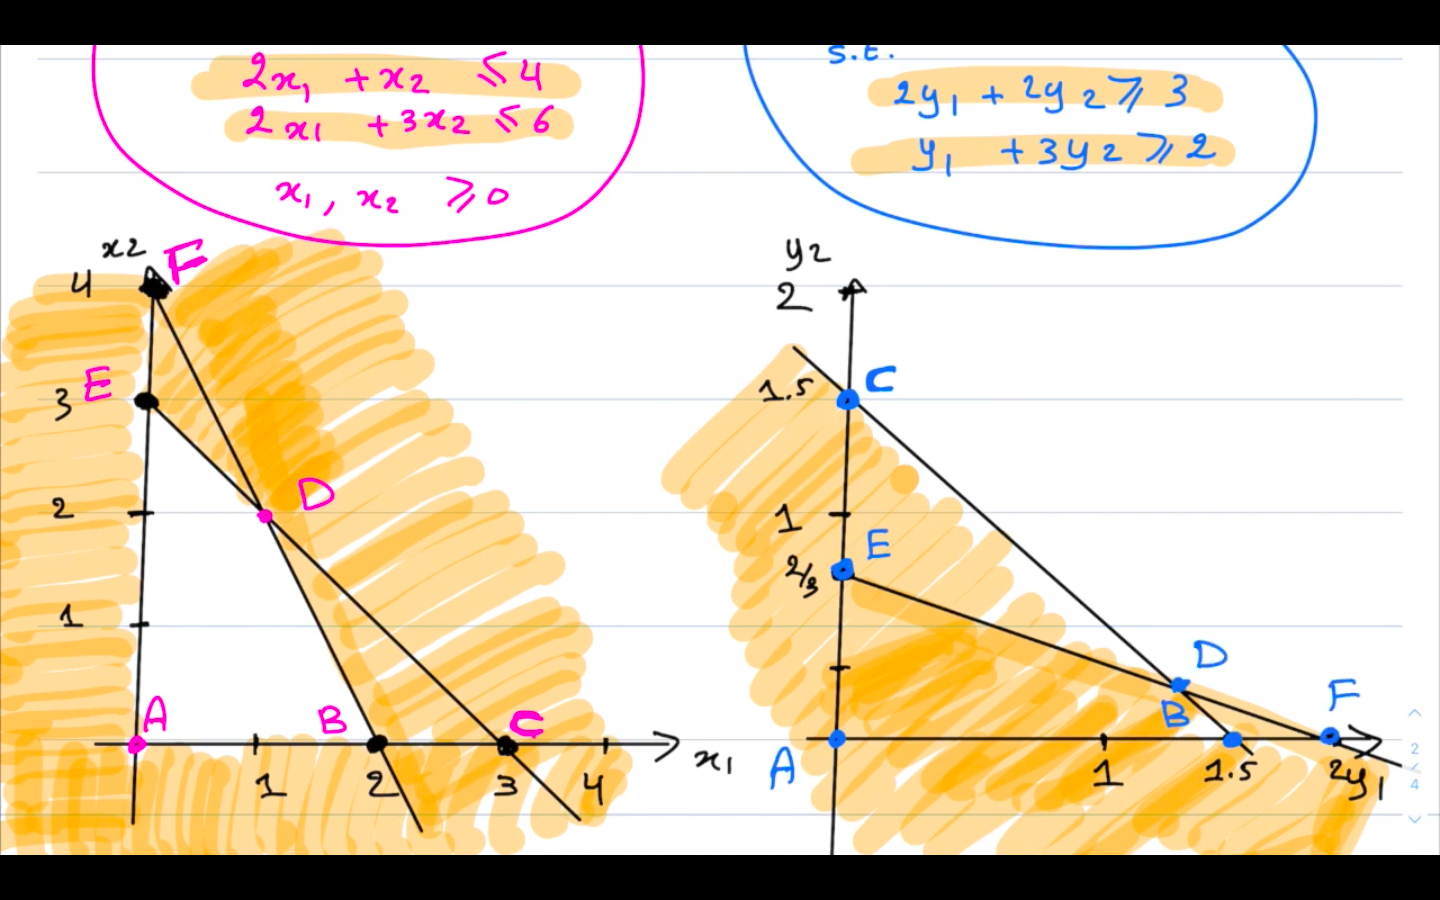
\includegraphics[width=0.8\linewidth]{answer1.png}\end{center}}
\note{\begin{center}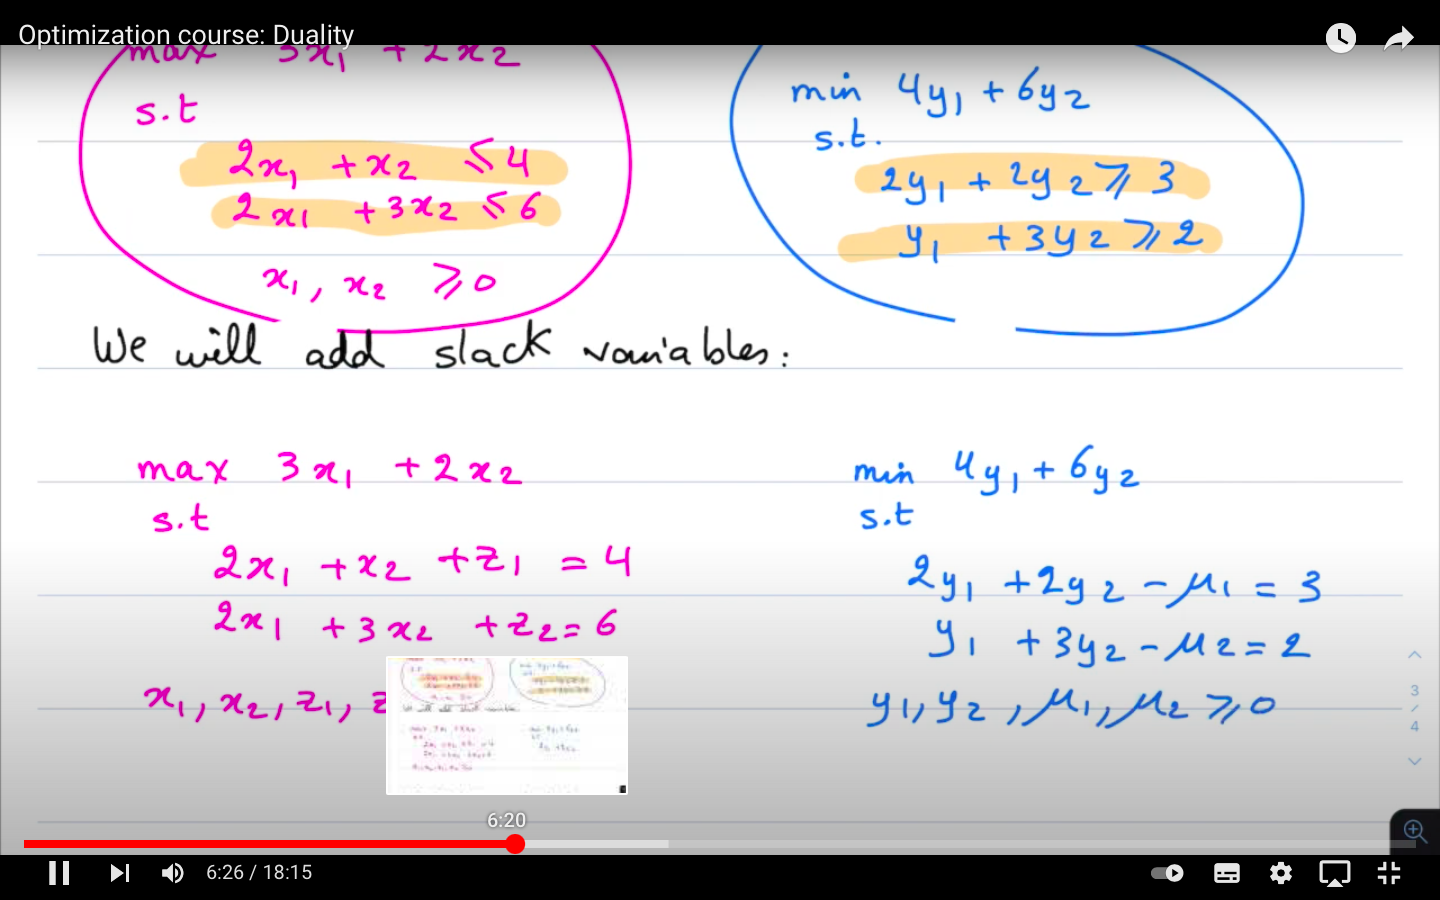
\includegraphics[width=0.8\linewidth]{answer3.png}\end{center}}
\note{\begin{center}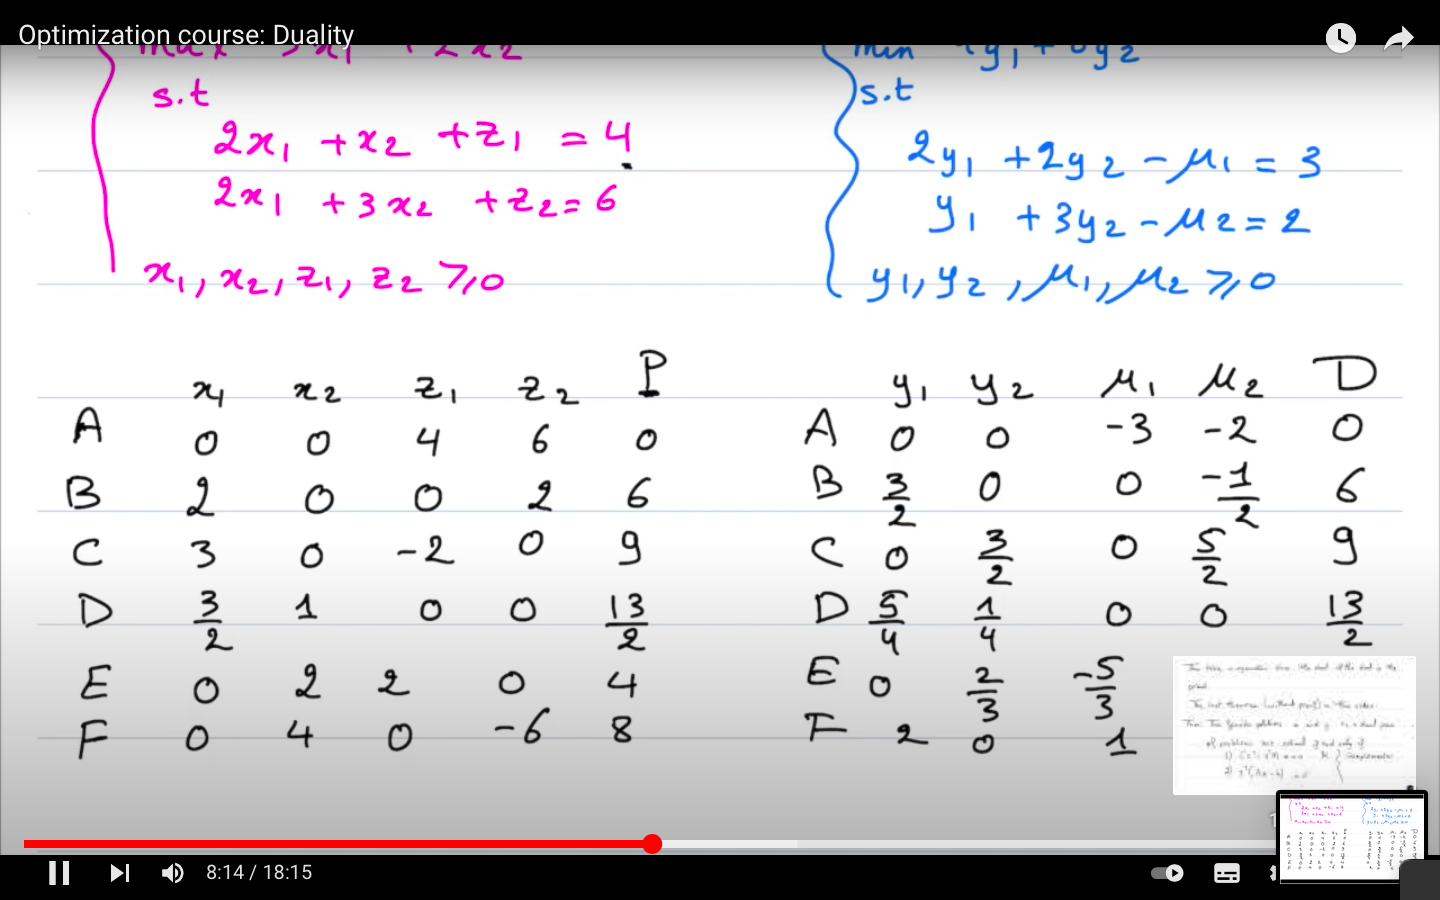
\includegraphics[width=0.8\linewidth]{answer2.png}\end{center}}
\note{\begin{center}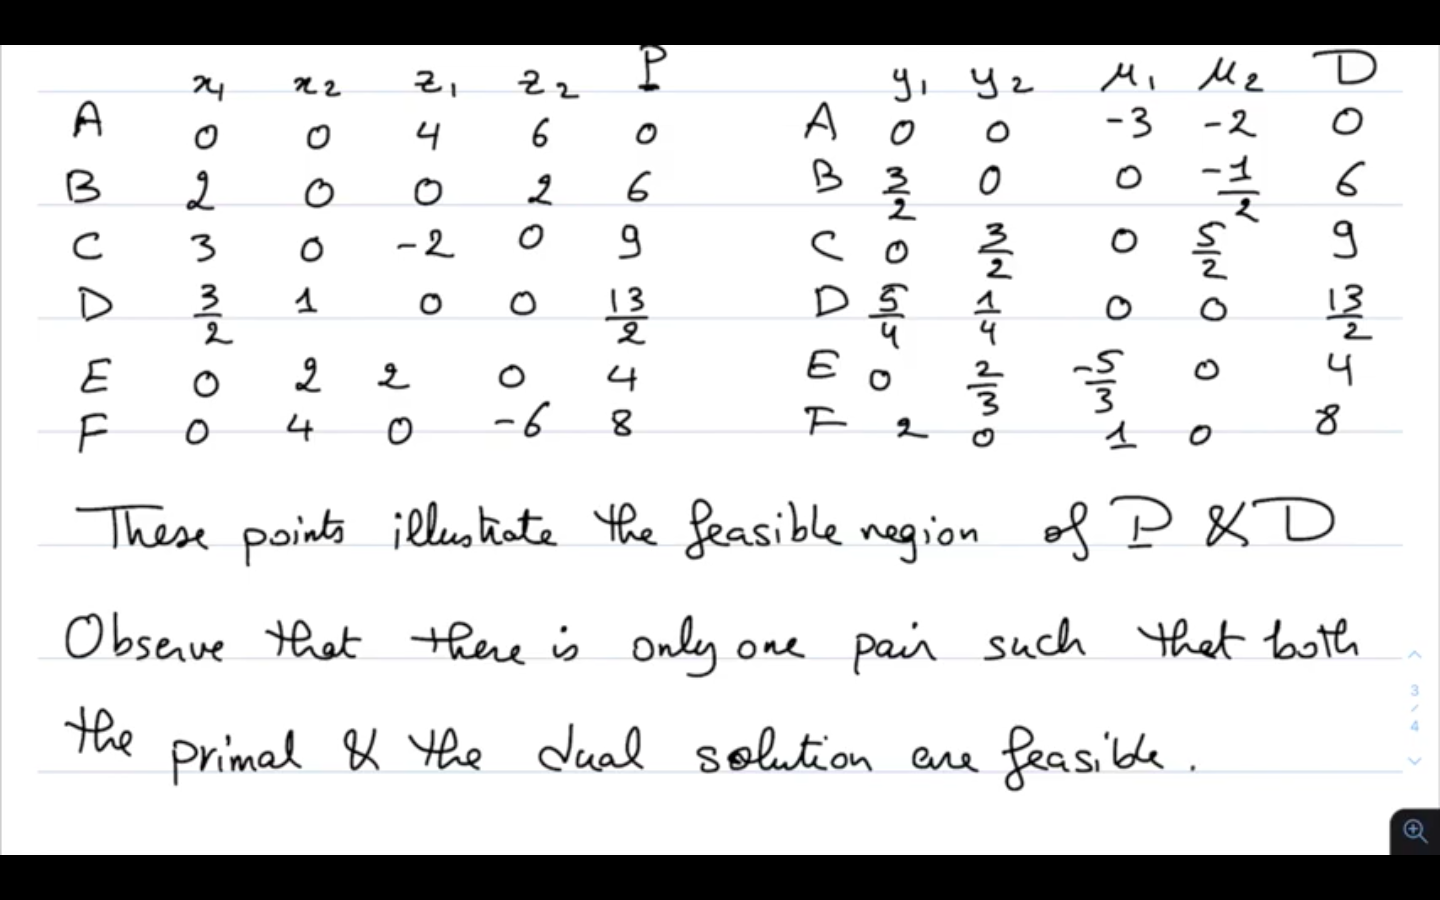
\includegraphics[width=0.8\linewidth]{answer4.png}\end{center}}

\begin{frame}{}
\begin{Exercise}
  Find the dual problem of
  \begin{equation*}
  \begin{aligned}
    \text{minimize } \quad & 4x_1 +4x_2+x_3 \\
    \text{subject to }\quad &
    \left\{
    \begin{array}{rcl}
      x_1+x_2+x_3 &\leq &2 \\
      2x_1+x_2 &= &3 \\
      2x_1+x_2+3x_3 &\geq &3 \\
      x_1,x_2,x_3 &\geq& 0
    \end{array}
    \right.
  \end{aligned}
\end{equation*}
Trick: normalize the problem first: eg $2x_1+x_2=3 \rightarrow \begin{cases}2x_1+x_2 \geq 3\\2x_1+x_2\leq 3\end{cases}$.
\end{Exercise}
\end{frame}
\note{
\url{https://www.youtube.com/watch?v=wVnr1HhUCT0}
}

\section{Some theory}

\begin{frame}{Dual of the dual}
\begin{theorem}
  In the case of linear programming, the dual of the dual is the primal.
\end{theorem}
\begin{proof}
 \[
\begin{rcases}
\text{max }\quad\uvec{b}^t \uvec{y}\\
\text{subject to }\quad A^t\uvec{y}\leq \uvec{c}, \forall y_i\geq0
\end{rcases} \text{DUAL}
\]
is equivalent to
\[
\begin{rcases}
\text{min }\quad-\uvec{b}^t \uvec{y}\\
\text{subject to }\quad -A^t\uvec{y}\geq -\uvec{c}, \forall y_i\geq0
\end{rcases} \text{DUAL}
\]
where, by taking again the Dual, leads to the original Primal.
\end{proof}
\end{frame}

\begin{frame}[allowframebreaks]{Meaning of Duality}
  Let us retake the example we saw in the last session:

  \begin{equation*}
    \begin{aligned}
      \text{maximize } \quad & z = 8x_1+5x_2 \\
      \text{subject to }\quad &
      \begin{array}{rcl}
        x_1 &\leq &150 \\
        x_2 &\leq &250 \\
        2x_1+x_2 &\leq &500 \\
        x_1,x_2 &\geq& 0
      \end{array}
    \end{aligned}
  \end{equation*}

  We found out that, from the initial tableau:

\begin{equation*}
\begin{array}{cc}
&\\
&z \\
\rightarrow &s \\
&t \\
&u\\
\mathrm{basic}
\end{array}
%
\begin{array}{c|ccccc|c}
  z & x_1 & x_2 & s & t & u & b \\ \hline
  1 & -8 & -5 & 0 & 0 & 0 & 0 \\ \hline
  0 & 1 & 0 & 1 & 0 & 0 & 150  \\
  0 & 0 & 1 & 0 & 1 & 0 & 250 \\
  0 & 2 & 1 & 0 & 0 & 1 & 500 \\
    & \uparrow & & & & &
\end{array}
%\end{matrix}
\end{equation*}

and after applying the different steps of the Simplex method we ended up with the final tableau:

  \begin{equation*}
  \begin{array}{cc}
  &\\
  R_1+5R_4&z \\
  &x_1 \\
  \rightarrow R_3-R_4&s \\
  &x_2\\
  &\mathrm{basic} \\
  \end{array}
  \begin{array}{c|ccccc|c}
    z & x_1 & x_2 & s & t & u & b \\ \hline
    1 & 0 & 0 & 0 & 1 & 4 & 2250 \\ \hline
    0 & 1 & 0 & 0 & -1/2 & 1/2 & 125  \\
    0 & 0 & 0 & 1 & 1/2 & -1/2 & 25 \\
    0 & 1 & 0 & 1 & 0 & 0 & 250 \\
      &  & & \uparrow& & &
  \end{array}
  \end{equation*}

Now, if we multiply the original availability of each resource (shown in the original tableau) by its marginal worth (taken from the final tableau) and get the sum, we obtain the optimal objective function value:

\[
z* = 2250 = 0(150)+1(250)+4(500)
\]

\end{frame}

\begin{frame}{Duality properties}


\begin{theorem}[Weak Duality]
  In a max LP, the value of primal objective function for any feasible solution is bounded from above by any feasible solution to its dual:
  \[\text{max } \qquad \bar{z} \leq \bar{w} \]
\end{theorem}
The statement is analogous to a minimization problem.
\begin{theorem}[Unboundness property]
  If primal (dual) problem has an unbounded solution, then the dual (primal) is unfeasible.
  \[\text{max } \qquad \bar{z} \leq \infty \]
\end{theorem}
\end{frame}

\begin{frame}[allowframebreaks]{Duality properties}


\begin{theorem}[Strong Duality]
  If the primal problem has an optimal solution,
  \[
  x^* = (x_1^*, \ldots, x_n^*)
  \]
  then the dual also has an optimal solution,
  \[
  y^* = (y_1^*, \ldots, y_m^*)
  \]
and
\[
z^* := \sum_j c_j x_j^* = \sum_i b_i y_i^* := w^*
\]

\end{theorem}
Thus: if feasible objective function values are found for a primal and dual pair of problems, and if these values are equal to each other, then both of the solutions are optimal solutions.

The Shadow prices that appear at the top of the optimal tableau of the primal problem are precisely the optimal values of the dual variables!
\end{frame}

\begin{frame}{A useful table}
  For any two given LP problems:
\begin{table}
  \begin{tabular}{c|c|c|c}
    Primal / Dual & not feasible & unbounded  & has a solution \\\hline
    not feasible & possible & possible & no \\\hline
    unbounded & possible & no & no \\\hline
    has a solution & no & no & same values\\
  \end{tabular}
\end{table}
The simplex algorithm solves the primal and dual problems simultaneously.
\end{frame}

\begin{frame}{Cases with no optimal solutions for primal and dual}
  Exactly one of the following mutually exclusive cases always occurs:
  \begin{itemize}
    \item Both primal and dual problems are feasible, and both have optimal (and equal) solutions.
    \item Both primal and dual problems are infeasible (have no feasible solution).
    \item The primal problem is feasible but unbounded, and the dual problem is infeasible.
    \item The dual problem is feasible but unbounded, and the primal problem is infeasible.
  \end{itemize}
\end{frame}

\section{Complementary slackness}

\begin{frame}[allowframebreaks]{Complementary slackness}
  Because each decision variable in a primal problem is associated with a constraint in the dual problem, each such variable is also associated with a slack or surplus variable in the dual.

  {\bf Variables in one problem are complementary to constraints in the other.}

  In any solution, if the primal variable is basic (with value $\geq0$, hence having slack, hence being non-binding), then the associated dual variable is non-basic ($=0$, hence having no slack, hence being binding), and viceversa.


  \begin{theorem}
    If in an optimal solution to a LP problem an inequality constraint is not binding, then the dual variable corresponding to that constraint has a value of zero in any optimal solution to the dual problem. 
  \end{theorem}
  
  \framebreak

  In other words: 
  \begin{itemize}
    \item if a variable is positive, then the associated dual constraint must be binding; or
    \item if a constraint fails to bind, than the associated variable must be zero; but recall that
    \item it is possible for a primal constraint to be binding while the associated dual variable is equal to zero (no slack in both primal and dual).
  \end{itemize}
  {\bf There cannot be slack in both a constraint and the associated dual variable.}
 
  \framebreak

  Suppose $x_0$ and $y_0$ are feasible solutions of (max) and (min) representations. Then, $x_0,y_0$ are optimal solutions if and only if
    \begin{eqnarray*}
      (b-Ax_0)\cdot y_0 =0\\
      (A^ty_0-c) \cdot x_0 =0
    \end{eqnarray*}
  
\end{frame}
\note{Veure exemple pràctic a \url{https://youtu.be/o1pznRt_-y0?t=1603}}

\begin{frame}[allowframebreaks]{Example: The diet problem}

  \begin{Exercise}
    You are feeding animals in a farm.Your animals have some basic requirements for nutrients, and you want to minimize the cost fulfilling those requirements. You need to know:
    \begin{enumerate}
      \item What foods do I have avaliable and which is each ones cost?
      \item What nutrients are needed and which is the nutrients content per food?
    \end{enumerate}
    Formulate the problem in an abstract way.
  \end{Exercise}
  \begin{Exercise}
    Come back to the previous problem, but now, there is a seller that tells you she has the pills you need to ensure the nutrients, forgetting about specific food. Reformulate the problem in terms of the maximum revenue the seller company wants. What is the price per pill to maximize her benefits, subject to the constraint that the pills are cheaper than the actual food.
  \end{Exercise}
  \begin{Exercise}
    Rationalize the complementarity slackness theorem within the context of the previous exercise. What does it mean to buy a positive quantity of the first food (primal LP problem) in terms of the constraint related to the first pill (dual problem)?
  \end{Exercise}
\end{frame}
  \note{Problema formulat a les notes I que tinc a material}
\begin{frame}{Using duality and CS to solve LP problems}
  \begin{Exercise}
    Just by checking the feasibility of the primal and dual problem for
    \begin{equation*}
      \begin{aligned}
        \text{maximize } \quad & z = x_1-x_2 \\
        \text{subject to }\quad &
        \begin{array}{rcl}
          -2x_1 +x_2 &\leq &2 \\
          x_1-2x_2 &\leq &2 \\
          x_1+x_2 &\leq &5 \\
          x_1,x_2 &\geq& 0
        \end{array}
      \end{aligned}
    \end{equation*}
    find what is the solution.
  \end{Exercise}
\end{frame}

\note{extret les notes duality. Comença per trobar els punts de creuament de les restriccions del p`rimal. Aleshores aplica CS per avaluar què passa al problema dual}

\section{References}
\begin{frame}{References}
    \footnotesize
    \begin{thebibliography}{99}
    \setbeamertemplate{bibliography item}[text]
      \begin{columns}[t]
        \begin{column}{.45\textwidth}
            \bibitem{carter} Michael W. Carter, Camille C. Price, and Ghaith Rabadi. Operations Research, 2nd Edition. CRC Press.
            \bibitem{harel} David Harel, with Yishai Feldman. Algorithmics: the spirit of computing, 3rd Edition. Addison-Wesley.
            \bibitem{rardin} Ronald L. Rardin. Optimization in Operations Research, 2nd Edition. Pearson.
            \bibitem{hefferon} J. Hefferon. \href{http://joshua.smcvt.edu/linearalgebra}{Linear algebra (4th Ed)}.
        \end{column}
        \begin{column}{.45\textwidth}
            \bibitem{riley} K.F. Riley, M.P. Hobson, S.J. Bence. Mathematical Methods for Physics and Engineering (2nd Ed). McGraw Hill.
            \bibitem{nocedal} J. Nocedal, S. J. Wright. Numerical Optimization (2nd Ed). Springer.
            \bibitem{beers} Kenneth J. Beers. Numerical methods for chemical engineering: applications in Matlab. Cambridge University Press.
            \bibitem{barber} D. Barber. Bayesian reasoning and machine learning. Cambridge University Press.
        \end{column}
      \end{columns}
    \end{thebibliography}
\end{frame}
%----------------------------------------------------------------------------------------

\end{document}
